\centerline{\bf \Huge Тренировочная олиммпиада}
\centerline{\bf \Huge 8 класс}

\begin{flushright}
        \scriptsize{}
\end{flushright}

\problem{1}
Может ли 2024-я степень числа оканчиваться на 2026?

\problem{2}Найдите натуральные решения уравнения:
\[ \dfrac{1}{x} + \dfrac{1}{y} = \dfrac{1}{1000}\]

\problem{3}
Найдите угол, отмеченный знаком вопроса. Изображенный треугольник равносторонний.

\begin{center}
    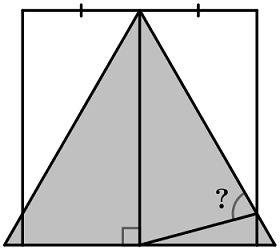
\includegraphics[width=0.2\textwidth]{ЭлМШ 2024-2025/II блок/Киви/Олимпиады/Olymp_8_1_2.png}
\end{center}

\problem{4}
Найдите сумму всех коэффициентов многочлена после раскрытия скобок и приведения подобных членов: $\left(x^2-3 x+4\right)^{10}\left(x^2-3 x+1\right)^{10}.$

\problem{5}
На эксклюзивную дегустацию дубайского шоколада съехались туристы из трех турфирм: «Хинкал-тур», «Папаха-тур» и «Тур-тур». Туристов из «Хинкал-тур» приехало в три раза меньше, чем из «Папаха-тур». Прежде чем дегустировать шоколад, туристы из каждой турфирмы обменялись рукопожатиями с туристами из других турфирм. Оказалось, что каждому туристу из «Хинкал-тур» пожали руку 11 раз, каждому туристу из «Тур-тур» - 6 раз, а каждому туристу из «Папаха-тур» - 5 раз. Докажите, что рукопожатий было не менее чем 157 , если известно, что туристов было 52.
